\documentclass[addpoints,12pt]{exam}
%\documentclass[12pt]{article}
\usepackage[letterpaper, margin=0.75in]{geometry}
\usepackage{graphicx}
\usepackage{enumitem}
\usepackage{booktabs}
\usepackage{tabularx}
\usepackage{amsmath}
\usepackage{color}

\begin{document}
\footer{}{Page \thepage\ of \numpages}{}

\begin{center}

\includegraphics[width=10cm]{../images/logo.png}
\end{center}

\begin{center}
\noindent{\LARGE Conceptual Physics \\ Homework Packet 3\\ Solutions \\}
\end{center}


 
\clearpage

\begin{flushright}
Score: \hspace{0.2in} / \numpoints ~ points
\end{flushright}


\begin{questions}
\question[4] 
\begin{parts}
\part Why do people mostly notice the gravitational force acting on their bodies if it is such a comparatively weak force?
\begin{TheSolution}
Gravity is the weakest force, however we are very close to a massive object (the Earth). We are also comparatively large to atoms and have lots of mass, so the force between us and the Earth is very noticeable. However, if we were floating in space and very very far away from distant object, we wouldn't notice gravity.
\end{TheSolution}

\part In what ways, if any, do we feel the other forces?
	\begin{TheSolution}
	The nuclear forces (both strong and weak) are short-range forces -- they act on a length-scale comparable to that of an atomic nucleus. People are so vastly larger than atomic nuclei that we don't notice this force.
	
	All contact forces (friction, push-back when we touch objects, etc.) are the result of the electromagnetic forces. If it wasn't for the repulsion between electrons when we stand on the ground, we would fall through to the center of the Earth.
	\end{TheSolution}
\end{parts}
	
	\question[4]
	Two satellites are orbiting the Earth. Satellite A has a mass of 100~kg, satellite B has a mass of 200~kg. If they are orbiting at the same distance from Earth, which (if any) experiences the greater gravitational force? Why? (I recommend you draw a diagram - but it's optional)
		\begin{TheSolution}
			The two satellite are orbiting at the same distance, however one is twice as massive as the other. Gravitational force between objects is proportional to mass. Since the Earth is the same to both satellites, this means that the larger satellite experiences the stronger force. Satellite B is twice as massive as satellite A, and so \textbf{Satellite B experiences the greater gravitational force} (specifically, it experiences twice the force).
		\end{TheSolution}
	
\question[4]
	You jump straight up in the air.
	\begin{parts}
		\part When do you have the greatest gravitational potential energy? When do you have the greatest kinetic energy?
			\begin{TheSolution}
			You have the largest gravitational potential energy when you are at the highest point -- at the top of the jump.
			
			All the potential energy was transformed form your initial kinetic energy. As you rise, you slow down. Therefore, you have the most kinetic energy at the bottom of your jump. If we assume energy is conserved, this would be at the beginning or the end (when you fist jump and when you hit the ground again). If energy isn't conserved (say, because you lost some energy to friction with the air) then you would have the most kinetic energy at the beginning. (Note: either answer will be marked as correct).
			\end{TheSolution}
		\part Assume your mass is 70~kg and you reach a maximum jumping height of 1.25~m. Prove that your initial velocity must have been at least 5~m/s up. (let $g = 10~m/s^2$. If you don't have a calculator, it may be easier to write 1.25~m as 5/4~m)
			\begin{TheSolution}
			There are multiple ways to prove this.
			\begin{itemize}
				\item One way is to simply derive the 5~m/s. All the potential energy at the end of the jump came from the kinetic energy at the beginning. The largest potential energy is:
			\begin{eqnarray}
			Initial~Kinetic~Energy &=& Largest~Potential~Energy \nonumber \\
			\frac{1}{2}mv^2 &=& mgh \nonumber \\
			\frac{1}{2}v^2 &=& gh \nonumber \\
			v^2 &=& 2gh \nonumber \\
			\Rightarrow v &=& \sqrt{2gh} \nonumber
			\end{eqnarray}
			Now that we have an algebraic expression for the velocity, we can use the height and acceleration due to gravity. Note: The mass was unnecessary information.
			\begin{eqnarray}
			v &=& \sqrt{2gh} \nonumber \\
			&=& \sqrt{2\times 10~m/s^2 \times 5/4~m} \nonumber \\
			&=& \sqrt{\frac{20\times 5}{4}m^2/s^2} \nonumber \\
			&=& \sqrt{25~m^2/s^2} \nonumber \\
			&=& 5~m/s \nonumber
			\end{eqnarray}
			
			\item Another way is to show that the initial kinetic energy for 5~m/s is equal to the potential energy at the height:
			\begin{eqnarray}
			Initial~Kinetic~Energy &=& \frac{1}{2}mv^2 \nonumber\\
			&=&\frac{1}{2}70~kg\times(5~ m/s)^2 = 875~kg~m/s^2\nonumber \\
			Largest~Potential~Energy &=& mgh \nonumber\\
			&=& 70~kg\times 5/4~m \times 10~m/s^2 = 875~m/s^2 \nonumber
			\end{eqnarray}
			These two numbers are the same, and so the 5~m/s would satisfy the condition.
			\end{itemize}
			In either case, you must have had at least the amount of kinetic energy corresponding to 5~m/s, since any less and you would have been moving slower and not rising as high. Any more could be explained by an energy loss (say, because of friction with the air).
			\end{TheSolution}
	\end{parts}	
\question[4]
	The Apollo spacecraft felt gravitational attractions from both the earth and the moon. Was there any time during the flight when \textbf{one} of these forces was zero? Could a place exist where the \textbf{net} force from the earth and the moon was zero? (From \textit{The Fundamental Interactions} handout, problem B4)
		\begin{TheSolution}
		The gravitational force of both the Earth and the moon extend out everywhere. If an object is very, very far away (say, on the other side of the galaxy) then the gravitational force would be minuscule but still not zero. Therefore, at no point would the spacecraft experience no force from the earth and the mooon.
		
		However, if the spacecraft is partway \textit{between} the earth and the moon, each pulling in opposite direction, then the two forces can cancel out and the \textit{net force} would be zero.
		\end{TheSolution}
	
\question[6]
	Tides arise from gravitational interactions between the Earth and the Moon. (\textit{High tides} are the state of the tide when at its highest level.) Because the Moon rotates about the Earth once every 28 days, the high tides to not occur at the same time each day. Also, the magnitude of the high tide will vary from day to day. To understand why, consider the positions of the Moon relative to the Sun and Earth below:
	\begin{center}
	\input{../images/hightides.pdf_tex}
	\end{center}
	\begin{parts}
		\part For which of these configurations will the high tide be the greatest? Please explain.
			\begin{TheSolution} \textbf{At points A and C.}
			
			At point A, both the moon and the sun are pulling on the oceans. They are adding together --  creating a large high tide. 
			
			When the moon orbits around the earth, it creates a tidal bulge on \textit{both} sides of the earth (1) at the point closest to the moon, because of gravity and (2) at the point \textit{directly opposite} (other side of the earth) because of the inertial momentum on the ocean from the earth and moon orbiting each other. The same is true with the sun and the earth (though the resulting effect is much smaller). Therefore, at point C the tidal bulges from the sun and moon \textit{still add together}.
			
			\begin{center}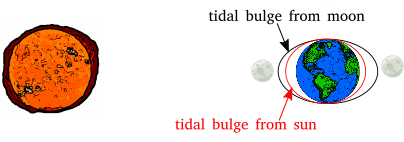
\includegraphics[width=0.5\textwidth]{../images/hightides_A.png}\end{center}
			\end{TheSolution}
		\part For which of these configuation with the high tide be the least? Please explain.
			\begin{TheSolution} \textbf{At points B and D.}
				Both the sun and moon create tidal on the earth. When these bulges are \textit{perpendicular} to each other, they cancel each other out rather than add together. Since the bulge from the moon is much larger, there is still a high tide, but it is not as large as it is for A and C.
				
				\begin{center}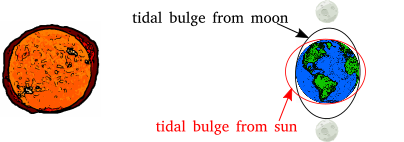
\includegraphics[width=0.5\textwidth]{../images/hightides_B.png}\end{center}
			\end{TheSolution}
		\part Describe the Sun's role in determining the magnitude of the high tides.
			\begin{TheSolution}
			Both the sun and the moon create tidal bulges on the earth. The one created by the moon is much larger, and so dominates when we see the tides. However, the bulge created by the sun can significantly add to the high tide, or lower it, depending on how the sun and moon align with the earth.
			\end{TheSolution}
	\end{parts}
		
	\question[4]
	\begin{parts}
		\part You release a magnet on a tabletop near a big piece of iron, and the magnet leaps across the table to the iron. Does the \textbf{magnetic potential energy} increase, or decrease? Explain.
		\begin{TheSolution}
		The magnet and iron are magnetically attracted to each other: the magnetic force in this case is \textit{attractive.} By holding the two apart, there is therefore stored potential energy, which is converted to kinetic energy as the two come together. Therefore, the magnetic potential energy \textit{decreases} in this scenario.
		\end{TheSolution}
		\part Suppose instead that you have two repelling magnets. You give them an initial push towards each other, so they decelerate while approaching each other. Does the \textbf{magnetic potential energy} increase, or decrease? Explain.
		\begin{TheSolution}
		The two magnetic are repelling each other, and so as they come together their kinetic energy is decreasing and being turned into potential energy. Therefore, the magnetic potential energy \textit{increases} in this scenario.
		\end{TheSolution}
	\end{parts}
	 
\end{questions}








\end{document}